\documentclass[a4paper,12pt]{article}

\usepackage{geometry}
\usepackage{polski}
\usepackage{amsmath}
\usepackage{makecell}
\usepackage{ragged2e}
\usepackage{hyperref}
\usepackage{array}
\usepackage{pdfpages}
\usepackage{xparse}
\usepackage{siunitx}
\usepackage{float}
\restylefloat{table}

\newenvironment{changemargin}[2]{%
\begin{list}{}{%
\setlength{\topsep}{0pt}%
\setlength{\leftmargin}{#1}%
\setlength{\rightmargin}{#2}%
\setlength{\listparindent}{\parindent}%
\setlength{\itemindent}{\parindent}%
\setlength{\parsep}{\parskip}%
}%
\item[]}{\end{list}}

\NewDocumentCommand{\DIV}{om}{%
  \IfValueT{#1}{\setcounter{#2}{\numexpr#1-1\relax}}%
  \csname #2\endcsname
}
\graphicspath{ {./} }

\hypersetup{
	colorlinks=true,
	linkcolor=black,
	filecolor=magenta,
	urlcolor=blue,
	citecolor=black
}

\urlstyle{same}

\geometry{
 a4paper,
 total={170mm,257mm},
 left=20mm,
 top=20mm,
 }
 
\pagenumbering{arabic}

\begin{document}
\begin{justify}

\begin{center}
\begin{scriptsize}
\begin{tabular}{ |m{2.5cm}|l|l|l|l|l| }
	\hline
	\makecell{Wydział: \\ FiIS} & \multicolumn{2}{|l|}{\makecell{Imię i nazwisko: \\ 1. Piotr Moszkowicz \\ 2. Wiktor Jasiński}}  & \makecell{Rok: \\ Drugi} & \makecell{Grupa: \\ PN 14:40} & \makecell{Zespół: \\ 1} \\
	\hline
	\textbf{PRACOWNIA FIZYCZNA WFiIS AGH} & \multicolumn{4}{|l|}{\makecell{Temat: Współczynnik lepkości }}  & \makecell{Nr ćwiczenia: \\ 13} \\
	\hline
	\makecell{Data wykonania: \\ 25.03.2019} & \makecell{Data oddania: \\ 1.04.2019} & \makecell{Zwrot do popr. \\ 8.04.2019} & \makecell{Data oddania: \\ 15.04.2019} & \makecell{Data zaliczenia \\ \,} & \makecell{OCENA \\ \,} \\
	\hline
\end{tabular}
\end{scriptsize}

\vspace{2cm}

\begin{Large}
\textbf{Ćwiczenie nr 13: Współczynnik lepkości }
\end{Large}

\end{center}

\vspace{0.5cm}
\textbf{Cel ćwiczenia:} \\
\indent Wyznaczenie współczynnika lepkości gliceryny metodą Stokesa, zapoznanie się z własnościami cieczy lepkiej. \cite{instrukcja} 
\end{justify}

\newpage

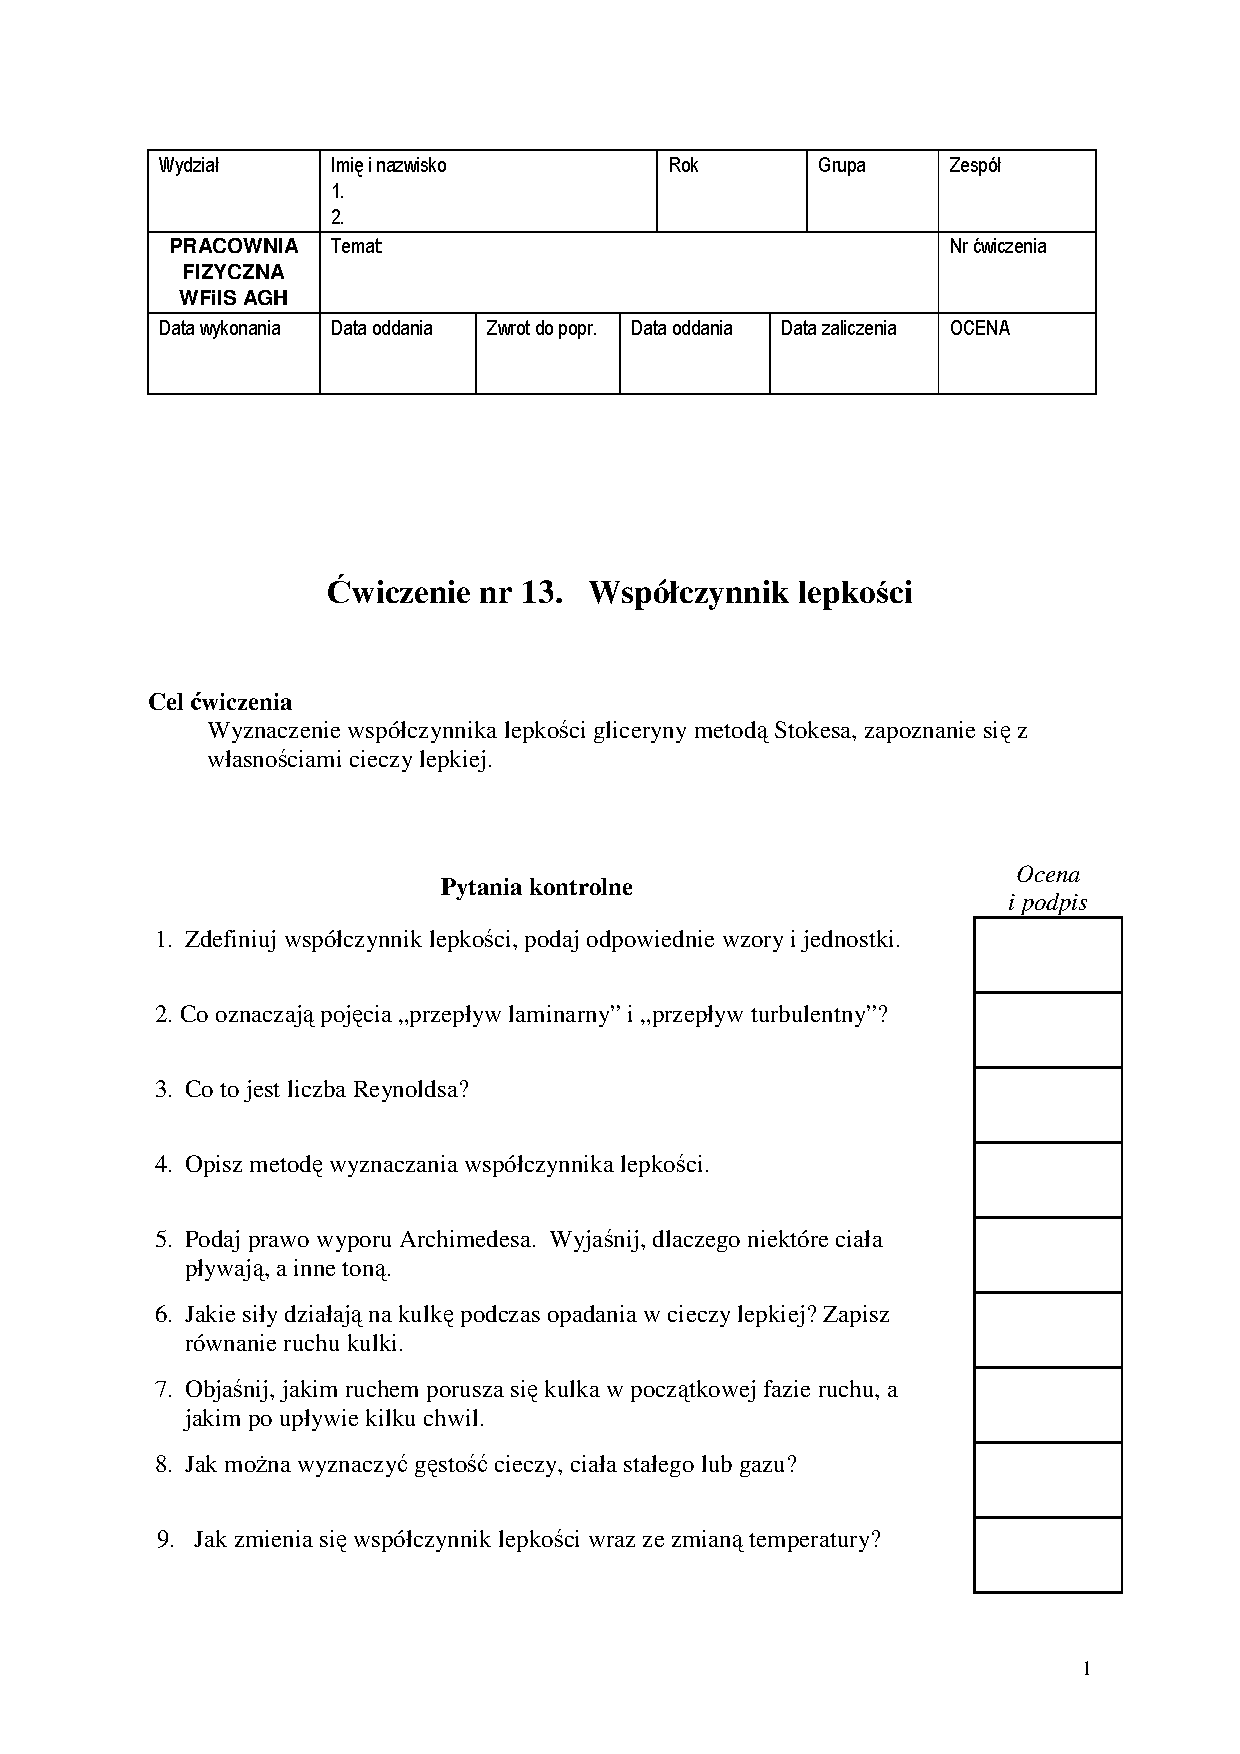
\includepdf[page={2}]{13_wykon}

\begin{justify}

\begin{enumerate}
\setcounter{enumi}{6}
\item Wyciągnij kulkę z cylindra poprzez kran umieszczony na jego dolnym końcu. Aby nie dopuścić do wylewania się gliceryny z cylindra należy posłużyć się zaciskaczem umieszczonym na wężyku. Gliceryna powinna ściekać do podstawionego pod wężykiem naczynia. Jeśli zachodzi potrzeba uzupełnienia gliceryny w cylindrze, należy przelać ją ostrożnie z naczynia lejąc po ściankach cylindra tak, aby wytworzyć jak najmniej pęcherzyków powietrza.
\item Po skończonych pomiarach należy zanotować temperaturę otoczenia, w której wykonywane było doświadczenie.
\end{enumerate}

\DIV[3]{section}{Wstęp teoretyczny}
\label{theory}

\subsection{Lepkość}
Właściwość płynów i plastycznych ciał stałych charakteryzująca ich tarcie wewnętrzne wynikające z przesuwania się względem siebie warstw płynu podczas przepływu (nie jest to natomiast opór przeciw płynięciu powstający na granicy płynu i ścianek naczynia, w warstwie granicznej.).  \cite{wspl}

\subsection{Przepływ laminarny}
Przepływ, który zachodzi przy małej prędkości, której prędkość graniczną możemy obliczyć na podstawie liczby Reynoldsa. Jest to przepływ uwarstwiony, w którym płyn w równoległych warstwach przepływa bez zakłóceń między nimi. \cite{pl}

\subsection{Przepływ turbulentny}
Przepływ, w którym jego parametry takie jak prędkość, ciśnienie i gęstość zmieniają się w sposób chaotyczny. \cite{pt}

\subsection{Liczba Reynoldsa}
Jedna z liczb podobieństwa stosowanych w mechanice płynów. Liczba ta pozwala oszacować występujący podczas ruchu płynu stosunek sił bezwładności do sił lepkości. \cite{reynolds} Wzór:
\begin{equation}
\label{wzr}
Re = \frac{v \cdot l \cdot \rho}{\eta}
\end{equation}

\subsection{Prawo Archimedesa}
Prawo Archimedesa głosi, że na ciało (częściowo lub całkowicie) zanurzone w płynie (cieczy, gazie lub plazmie) działa pionowa, skierowana ku górze siła wyporu $F_{w}$ której wartość jest równa ciężarowi płynu wypartego przez to ciało \cite{arch}:
\begin{equation}
F_{w} = m_{p} \cdot g = \rho_{g} \cdot g \cdot V
\end{equation}
gdzie:
\begin{align*}
m_{p} & \text{ - masa wypieranego płynu} \\
\rho_{g} &\text{ - gęstość płynu} \\
g & \text{ - przyspieszenie ziemskie} \\
V & \text{ - objętość wypieranego płynu}
\end{align*}

\section{Wyniki pomiarów}

\begin{align*}
\text{Droga spadania kulki: } & \Delta l = 820mm & u_{b}(\Delta l) = 2mm \\
\text{Średnica cylindra: } & D = 39mm & u_{b}(D) = 2mm \\
\text{Temperatura: } & Tmp = \SI{21.5}{\celsius} & u_{b}(Tmp) = \SI{1}{\celsius} \\
\text{Masa: } & & u_{b}(m) = 0.001g \\
\text{Średnica: } & & u_{b}(d) = 0.01mm \\
\text{Czas: } & & u_{b}(t) = 0.01s
\end{align*}

\begin{table}[H]
\begin{center}
\begin{scriptsize}
\begin{tabular}{|l|l|l|l|l|l|}
\hline
Nr. pomiaru &  Nr. kulki & Średnia kulki d [mm] & Masa kulki m [g] & Czas spadku kulki $\Delta t$ [s] & Wsp. lepkości $\eta$ [$Pa \cdot s$] \\
\hline
1 & 1 & 4.90 & 0.253  & 6.15 & 2.13 \\
2 & 1 & 4.90 & 0.253 & 6.19 & 2.15 \\
3 & 1 & 4.90 & 0.253 & 6.25  & 2.17 \\
4 & 1 & 4.90 & 0.253 & 6.14 & 2.13 \\
5 & 1 & 4.90 & 0.253 & 6.19 & 2.15 \\
\hline
6 & 2 & 3.98 & 0.175 & 7.66 & 2.16 \\
7 & 2 & 3.98 & 0.175 & 7.53 & 2.16 \\
8 & 2 & 3.98 & 0.175 & 7.54 & 2.15\\
9 & 2 & 3.98 & 0.175 & 7.59 & 2.16 \\
10 & 2 & 3.98 & 0.175 & 7.56 & 2.17 \\
\hline
11 & 3 & 3.96 & 0.110 & 9.68  & 2.60 \\
12 & 3 & 3.96 & 0.110 & 9.69 & 2.56\\
13 & 3 & 3.96 & 0.110 & 9.75 & 2.56\\
14 & 3 & 3.96 & 0.110 & 9.72 & 2.58 \\
15 & 3 & 3.96 & 0.110 & 9.60 & 2.57 \\
\hline
16 & 4 & 4.88 & 0.254 & 6.12 & 2.07 \\
17 & 4 & 4.88 & 0.254 & 6.12 & 2.09 \\
18 & 4 & 4.88 & 0.254 & 6.10 & 2.07 \\
19 & 4 & 4.88 & 0.254 & 6.12 & 2.08\\
20 & 4 & 4.88 & 0.254 & 6.15 & 2.09 \\
\hline
21 & 5 & 4.98 & 0.259 & 9.68 & 1.71 \\
22 & 5 & 4.98 & 0.259 & 9.69 & 1.71 \\
23 & 5 & 4.98 & 0.259 & 9.75 & 1.72 \\
24 & 5 & 4.98 & 0.259 & 9.72 & 1.72 \\
25 & 5 & 4.98 & 0.259 & 9.60 & 1.70 \\
\hline
\end{tabular}
\caption{Wyniki pomiarów i obliczonych wartości $\eta$ dla kolejnych kulek }
\label{table:1}
\end{scriptsize}
\end{center}
\end{table}

\begin{table}[H]
\begin{center}
\begin{scriptsize}
\begin{tabular}{|l|l|}
\hline
Nr. kulki & Wsp. lepkości $\eta$ [$Pa \cdot s$] \\
\hline
1 & 2.14 \\
\hline
2 & 2.16 \\
\hline
3 & 2.57 \\
\hline
4 & 2.08 \\
\hline
5 & 1.71 \\
\hline
\end{tabular}
\caption{Wartości średnia współczynnika lepkości dla każdej z kulek }
\label{table:2}
\end{scriptsize}
\end{center}
\end{table}

\paragraph{Wartość średnia współczynnika lepkości $\eta$ = 2.13$Pa \cdot s$}
\paragraph{Niepewność typu A: $u_{A}(\eta)$ = 0.28$Pa \cdot s$}
\paragraph{Niepewność złożona typu B: }
\begin{changemargin}{-2cm}{-2cm}
\begin{align*}
u_{c}(\eta) = \sqrt{[\frac{\partial \eta}{\partial m} \cdot u(m)]^2 + [\frac{\partial  \eta}{\partial \rho} \cdot u(\rho)]^2 + [\frac{\partial \eta}{\partial d} \cdot u(d)]^2 + [\frac{\partial \eta}{\partial g} \cdot u(g)]^2 + [\frac{\partial \eta}{\partial t} \cdot u(t)]^2 + [\frac{\partial \eta}{\partial l} \cdot u(l)]^2 + [\frac{\partial \eta}{\partial D} \cdot u(D)]^2}  \\ = 0.16 Pa \cdot s
\end{align*}
\end{changemargin}
\paragraph{Przy liczeniu niepewności rozszerzonej ustalamy k = 2, oraz mnożymy $u_{A}$, gdyż jest większe.}
\paragraph{Niepewność rozszerzona: $U(\eta)$ = $2 \cdot u_{A}(\eta)$ = 0.56 $Pa \cdot s$}
\paragraph{Prędkość spadania kulki nr. 4  $ v = \frac{\Delta l}{\Delta t}$ =  133.33$\frac{mm}{s}$}
\paragraph{Niepewność złożona typu B: $u_{b}(v)$ = $\sqrt{[\frac{\partial v}{\partial l} \cdot u(l)]^2 + [\frac{\partial v}{\partial t} \cdot u(t)]^2}$  = 2.182$\frac{mm}{s}$}
\paragraph{Niepewność rozszerzona: $U(v)$ = $ 2 \cdot u_{b}(v)$ = 4.36$\frac{mm}{s}$}
\paragraph{Liczba Reynoldsa dla kulki nr. 4:  $R$ = 0.39 (obliczona ze wzoru \ref{wzr})}
\paragraph{Niepewność złożona typu B: $u_{b}(R)$ = $\sqrt{[\frac{\partial R}{\partial v} \cdot u(v)]^2 + [\frac{\partial R}{\partial l} \cdot u(l)]^2 + [\frac{\partial R}{\partial \rho} \cdot u(\rho)]^2 + [\frac{\partial R}{\partial \eta} \cdot u(\eta)]^2}$ = 0.0307}
\paragraph{Niepewność rozszerzona: $U(R)$ = $2 \cdot u_{b}(R)$ = 0.062}

\section{Wyniki}

Zgodnie z informacjami zamieszczonymi poniżej nasz pomiar biorąc pod uwagę niepewność pomiarową jest zgodny z wartością tablicową: \\
\begin{center}
$|\eta - \eta_{dosw}| < u(\eta)$ \\
$|1.945 - 2.13| < 0.32$ \\
$0.185 < 0.32$
\end{center}

\begin{table}[H]
\begin{center}
\begin{scriptsize}
\begin{tabular}{|c|c|}
\hline
Wsp. lepkości $\eta$ [$Pa \cdot s$] & Niepewność rozszerzona $U(\eta)$ [$Pa \cdot s$] \\
\hline
2.13 & 0.56  \\
\hline
\end{tabular}
\caption{Zestawienie wyników}
\label{table:3}
\end{scriptsize}
\end{center}
\end{table}

\section{Bibliografia}

\begingroup
\renewcommand{\section}[2]{}%
\begin{thebibliography}{}
\bibitem{instrukcja} \url{http://www.fis.agh.edu.pl/~pracownia_fizyczna/cwiczenia/13_wykon.pdf}
\bibitem{wspl} \url{https://pl.wikipedia.org/wiki/Lepko%C5%9B%C4%87}
\bibitem{pl} \url{https://pl.wikipedia.org/wiki/Przep%C5%82yw_laminarny}
\bibitem{pt} \url{https://encyklopedia.pwn.pl/haslo/przeplyw-turbulentny;3963563.html}
\bibitem{arch} \url{https://pl.wikipedia.org/wiki/Prawo_Archimedesa}
\bibitem{reynolds} \url{https://pl.wikipedia.org/wiki/Liczba_Reynoldsa}
\end{thebibliography}
\endgroup

\end{justify}

\end{document}